\documentclass{beamer}
 
\usepackage[utf8]{inputenc}
\usepackage{graphicx}
\usepackage[font={footnotesize}]{caption}
\usepackage{textcomp}
\usepackage{booktabs}
\usepackage{listings}
\lstset{language=C++,basicstyle=\footnotesize\ttfamily,keywordstyle=\color{red}}
\newcommand{\textapprox}{\raisebox{0.5ex}{\texttildelow}}
\setcounter{tocdepth}{2}
\setbeamertemplate{navigation symbols}{}
\usetheme{Luebeck}

\newcommand\pro{\item[$+$]}
\newcommand\con{\item[$-$]}
%-------------------------------------------------------
%	TITLE PAGE
%-------------------------------------------------------
\title[Geant4-GPU (McMaster University)]{Running Geant4 Functions on a GPU}
\subtitle{Discussion of Results}
\institute{McMaster University}
\author[S. Douglas, R. Gorrie, M .Pagnan, V. Reginato]{
Stuart Douglas -- dougls2
\\Rob Gorrie -- gorrierw
\\Matthew Pagnan -- pagnanmm
\\Victor Reginato -- reginavp
}
 
\begin{document}

\frame{\titlepage}
\begin{frame}
\frametitle{Overview}
\tableofcontents
\end{frame}

% =================== Section =================== 
\section{Introduction} 

\subsection{Brief Project Overview}
\begin{frame}
\frametitle{Brief Project Overview}
Take an existing particle simulation toolkit - Geant4 - and have some functions run on a GPU device to improve performance.
\end{frame}

\subsection{Explanation of Terms}
\begin{frame}
\frametitle{What is Geant4?}
\begin{itemize}
\item Geant4 is a toolkit that is meant to simulate the passage of particles through matter. 
\item It has been developed over the years through collaborative effort of many different institutions and individuals. 
\item Geant4's diverse particle simulation library has a wide variety of applications including
\begin{itemize}
\item High energy physics simulations
\item Space and radiation simulations
\item Medical physics simulations
\end{itemize}
\end{itemize}
\end{frame}

\begin{frame}
\frametitle{Demonstration}
\begin{center}
\emph{Demonstration -- Running Geant4 on the CPU}

\emph{Hadr04 With Visualization}
\end{center}
\end{frame}

\begin{frame}
\begin{itemize}
\frametitle{What is GP-GPU Computing?}
\item General-purpose graphic-processing-unit computing is a re-purposing of graphics hardware
\item Allows GPUs  to perform computations that would typically be computed on the CPU
\item If a particular problem is well suited to parallelization, GP-GPU computing can greatly increase performance
\end{itemize}
\end{frame}

\subsection{Scope}
\begin{frame}
\begin{itemize}
\frametitle{Scope}
\item Make current CPU functions available for use on GPU
\begin{itemize}
\item Add appropriate prefixes to function definitions
\item Make use of multiple parallel threads to execute each function
\end{itemize}
\item Ensure correctness of each GPU available function by matching results to the corresponding CPU function
\item Compare performance of GPU available functions to CPU functions
\end{itemize}
\end{frame}

\begin{frame}
\frametitle{Possible Implementations}
There were initially five possible implementations to reach 
a solution:
\begin{itemize}
\item Port Geant4 to the GPU such that each particle runs in parallel
\item Port all the functions of some class(es) to the GPU, with those functions privatized to the GPU
\item Port some functions of some class(es) to the GPU, memory stored on host, passing mem to device as necessary
\item Port some functions of some class(es) to the GPU, memory stored and updated on host and device
\item Port some functions of some class(es) to the GPU, data divided between host and device, passing mem as necessary
\end{itemize}
\end{frame}

\begin{frame}
\frametitle{Solution Choice}
\begin{itemize}
\item Implementation 1 was believed to be unreasonable given schedule/resource limitations
\item Implementation 5 was found to be most suitable
\begin{itemize}
\item Easy to switch between CPU \& GPU versions
\item Less memory usage than other implementations
\item Least redundancy in computation
\end{itemize}
\end{itemize}
\end{frame}

\subsection{Purpose}
\begin{frame}
\begin{itemize}
\item Determine if target functions are suitable to parallelization 
\item Increase performance of functions when run on GPU
\item Decrease time required to run simulations involving ported functions
\end{itemize}
\frametitle{Purpose}
\end{frame}

% =================== Section =================== 
\section{Features}
\begin{frame}
\frametitle{Features}
\begin{itemize}
\item GPU acceleration available on an ``opt-in'' basis
\item Easy to enable/disable GPU acceleration
\item If GPU acceleration is enabled, some methods will run on GPU
\item Same results whether acceleration enabled or disabled
\end{itemize}
\end{frame}

\subsection{Easily Enable/Disable GPU Acceleration}
\begin{frame}
\frametitle{Easily Enable/Disable GPU Acceleration}
\begin{itemize}
\item Existing projects can use GPU acceleration without having to change any code 
\item Flag during build phase enables/disables GPU acceleration
\item Interface remains the same\footnote{implementation 1 only}, acceleration happens ``invisibly''
\end{itemize}
\end{frame}

\begin{frame}
\frametitle{Demonstration}
\begin{center}
\emph{Demonstration -- Enabling CUDA Acceleration}
\end{center}
\end{frame}

\begin{frame}[fragile]
\frametitle{Easily Enable/Disable GPU Acceleration}
Method calls to \texttt{G4ParticleHPVector} forwarded to GPU-based implementation
\begin{itemize}
\item This decision is made at compile time based on \texttt{cmake} flag
\end{itemize}

\begin{block}{Example of Forwarding Method Calls}
\begin{lstlisting}
inline G4double GetY(G4double x)
{
  #if GEANT4_ENABLE_CUDA
    return cudaVector->GetXsec(x);
  #else
    return GetXsec(x);
  #endif
}
\end{lstlisting}
\end{block}
\end{frame}

\begin{frame}
\frametitle{Accelerating Module on GPU}
Existing module \texttt{G4ParticleHPVector} ported to GPU using CUDA\\~\\

\begin{block}{Definition: CUDA}
CUDA is a GP-GPU programming model developed by NVIDIA, for use with NVIDIA graphics cards
\end{block}
\end{frame}

\begin{frame}
\frametitle{Why \texttt{G4ParticleHPVector}?}
\begin{itemize}
\item Represents empirically-found probabilities of collisions for different particles based on their energy
\item Identified as starting point by relevant stakeholders
\begin{itemize}
\item Used heavily in simulations run by stakeholders
\end{itemize}
\item Seems well-suited to parallelization
\begin{itemize}
\item Based on large vector of 2D points
\item Performs calculations over this vector
\item Sorted by x-value (particle energy)
\end{itemize}
\end{itemize}
\end{frame}

\begin{frame}
\frametitle{Two Implementations}
\begin{enumerate}
\item Forward all calls to existing \texttt{G4ParticleHPVector} interface to a GPU-based implementation of the module

\begin{itemize}
\item Store data vector in GPU memory
\item Copy results back to the CPU to return to the caller
\end{itemize}

\item Add new methods to \texttt{G4ParticleHPVector} interface that are well-suited to GPU computing
\begin{itemize}
\item Copy data vector to GPU memory on method call
\item Existing \texttt{G4ParticleHPVector} methods unchanged, continue to run on CPU
\end{itemize}
\end{enumerate}
\end{frame}

\subsection{Impl. 1: Existing Module in GPU Memory}
\begin{frame}
\frametitle{Impl. 1: Existing Module in GPU Memory}
Calls to \texttt{G4ParticleHPVector} forwarded to new GPU-based class\\~\\ % hack to get new line in Beamer

\textbf{Pros:}
\begin{itemize}
\pro Do not have to maintain a copy of the vector on the CPU
\pro Do not have to maintain a hashed vector
\pro Reduces how much is being copied to the GPU
\end{itemize}
\textbf{Cons:}
\begin{itemize}
\con All methods are run on the GPU
\end{itemize}
\end{frame}

\begin{frame}
\frametitle{Demonstration}
\begin{center}
\emph{Demonstration -- Running Geant4 on the GPU}

\emph{Hadr04 With Visualization}

\end{center}
\end{frame}

\subsubsection{Implementation of Select Methods on GPU}
\begin{frame}[fragile]
\frametitle{Impl. 1 -- \texttt{Times}}
\begin{block}{Times\_CUDA}
\begin{lstlisting} 
int tid = blockDim.x * blockIdx.x + threadIdx.x;
if (tid < nEntries) 
   theData[tid].xSec = theData[tid].xSec * factor;    
\end{lstlisting}
\end{block}
\end{frame}

\begin{frame}[fragile]
\frametitle{Impl. 1 -- \texttt{GetXSec}}
\begin{block}{GetXSec\_CUDA}
\begin{lstlisting}
int start = (blockDim.x * blockIdx.x + threadIdx.x);
for (int i = start; i < nEntries; i += numThreads) 
   if (theData[i].energy >= e) {
      resultIndex = Min(resultIndex, i);
      return;
      }
\end{lstlisting}
\end{block}
\end{frame}

\subsubsection{Impl. 1: Performance}
\begin{frame}
\frametitle{Impl. 1: Performance Results Summary}
\begin{itemize}
\item Most methods slower on GPU until \textapprox 10,000 entries in data vector
\item Most \emph{commonly-used} methods significantly slower on GPU, even with large data vector
\begin{itemize}
\item Lots of data accesses
\end{itemize}
\item Many problems in vector class not well-suited to parallelism
\end{itemize}
\end{frame}

\begin{frame}
\frametitle{Impl. 1: Performance Results -- \texttt{Times}}
\begin{itemize}
\item Multiplies each point in vector by factor
\end{itemize}
\begin{figure}
\centering
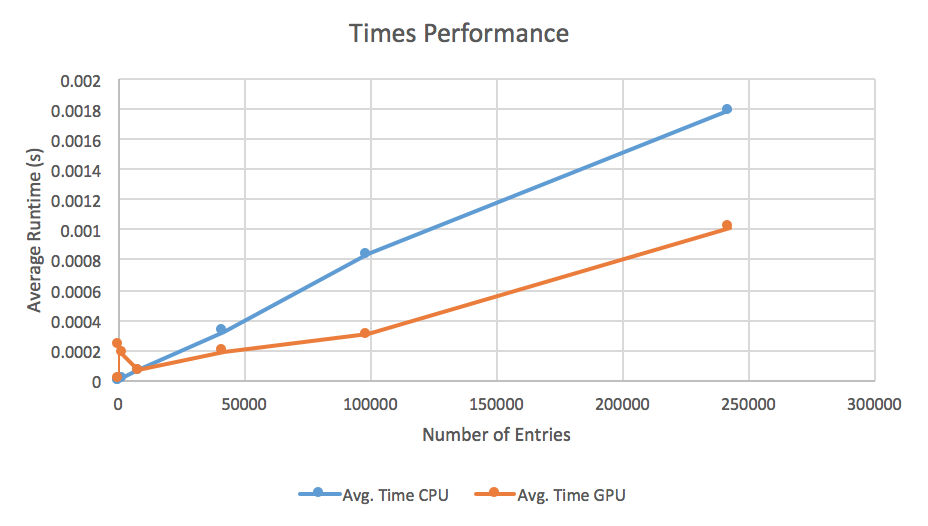
\includegraphics[width=0.8\textwidth]{images/times_line.png}
\caption{Runtime vs. Number of Data Points -- \texttt{Times}}
\end{figure}
\end{frame}

\begin{frame}
\frametitle{Impl. 1: Performance Results -- \texttt{GetXSec}}
\begin{figure}
\centering
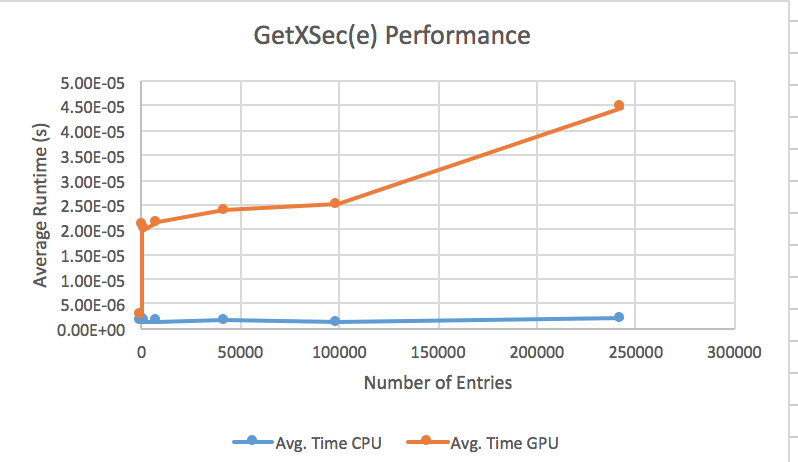
\includegraphics[width=0.8\textwidth]{images/getxsec_e_line.png}
\caption{Runtime vs. Number of Data Points -- \texttt{GetXSec}}
\end{figure}
\end{frame}

\begin{frame}
\frametitle{Impl. 1: Performance Results -- \texttt{SampleLin}}
\begin{figure}
\centering
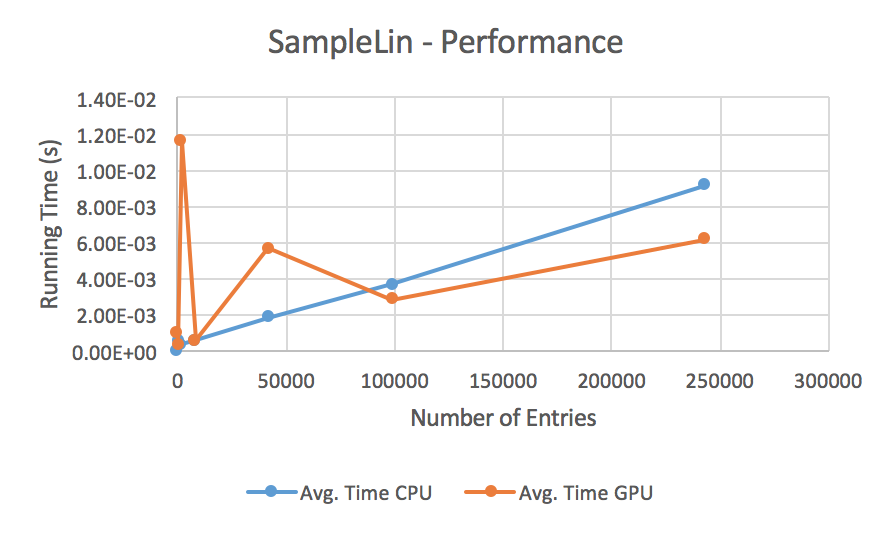
\includegraphics[width=0.8\textwidth]{images/samplelin_line.png}
\caption{Runtime vs. Number of Data Points -- \texttt{SampleLin}}
\end{figure}
\end{frame}

\begin{frame}
\frametitle{Impl. 1: Performance Results -- System Tests}
System Test \#1:
\begin{table}
	\begin{tabular}{lll}
	\toprule
	\bf CPU Time&\bf  GPU Time&\bf Speedup of GPU\\\midrule
	54.55s&72.08s&-1.32$\times$\\\bottomrule
	\end{tabular}
	\caption{Performance - Water, 2000 events}
\end{table}
System Test \#2:
\begin{table}
	\begin{tabular}{lll}
	\toprule
	\bf CPU Time&\bf  GPU Time&\bf Speedup of GPU\\\midrule
	54.55s&72.08s&-1.32$\times$\\\bottomrule
	\end{tabular}
	\caption{Performance - Uranium, 2000 events}
\end{table}
\end{frame}

\begin{frame}
\frametitle{Impl. 1: Performance Results -- System Tests (Cont.)}
System Test \#3:
\begin{table}
	\begin{tabular}{lll}
	\toprule
	\bf CPU Time&\bf  GPU Time&\bf Speedup of GPU\\\midrule
	54.55s&72.08s&-1.32$\times$\\\bottomrule
	\end{tabular}
	\caption{Performance - Water, 2000 events}
\end{table}
System Test \#4:
\begin{table}
	\begin{tabular}{lll}
	\toprule
	\bf CPU Time&\bf  GPU Time&\bf Speedup of GPU\\\midrule
	54.55s&72.08s&-1.32$\times$\\\bottomrule
	\end{tabular}
	\caption{Performance - Uranium, 2000 events}
\end{table}\end{frame}

\begin{frame}
\frametitle{Impl. 1: Performance Discussion}
\begin{itemize}
\item Simple ``getters'' and ``setters'' now require copy from GPU to CPU memory
\item Current code calling \texttt{G4ParticleHPVector} more data-oriented than computation-oriented
\item Low \texttt{GetXSec} performance due to lack of \texttt{Hash} object on GPU to accelerate finding min index
\item Although some functions faster, rarely used in practice
\end{itemize}
\end{frame}

\subsection{Impl. 2: Add New GPU-Accelerated Methods to Interface}
\begin{frame}
\frametitle{Impl. 2: Add New GPU-Accelerated Methods to Interface}
Add new methods to \texttt{G4ParticleHPVector} interface that are well-suited to parallelism\\~\\

\textbf{Pros:}
\begin{itemize}
\pro Only methods that run faster on the GPU are implemented
\pro Not forced to run methods that run slowly on GPU
\end{itemize}

\textbf{Cons:}
\begin{itemize}
\con Will have to maintain two copies of the vector
\con More copying the vector to and from the GPU
\end{itemize}
\end{frame}

\begin{frame}
\frametitle{Impl. 2: \texttt{GetXSecList}}
\begin{itemize}
\item Fill an array of energies for which we want the cross section values for
\item Send the array to the GPU to work on
\item Each thread works on its own query(s)
\end{itemize}
\end{frame}

\begin{frame}[fragile]
\frametitle{Implementation -- \texttt{GetXSecList}}
\begin{block}{GetXSecList}
\begin{lstlisting}[language=C++,basicstyle=\ttfamily,keywordstyle=\color{red}]
stepSize = sqrt(nEntries);
i = 0;
e = queryList[threadID];
    
for (i = 0; i < nEntries; i += stepSize) 
   if (d_theData[i].energy >= e) 
      break;
\end{lstlisting}
\end{block}
\end{frame}

\begin{frame}[fragile]
\frametitle{Implementation -- \texttt{GetXSecList -- cont}}
\begin{block}{GetXSecList -- cont}
\begin{lstlisting}[language=C++, basicstyle=\ttfamily, keywordstyle=\color{red}]
i =  i - (stepSize - 1); 

for (; i < nEntries; i++) 
   if (d_theData[i].energy >= e) 
      break;
   
d_queryList[threadID] = i;
\end{lstlisting}
\end{block}
\end{frame}


\subsubsection{Impl. 2: Performance}
\begin{frame}
\frametitle{Impl. 2: Performance Results Summary}
Performance of implementation 2 also proved slower than 
original Geant4 implementations of ParticleHPVector
\begin{itemize}
\item Buffered implementation begins to taper off, but at a 
much slower rate than the original
\end{itemize}
\end{frame}

\begin{frame}
\frametitle{Impl. 2: Performance Results -- \texttt{GetXSecList}}
\begin{figure}
\centering
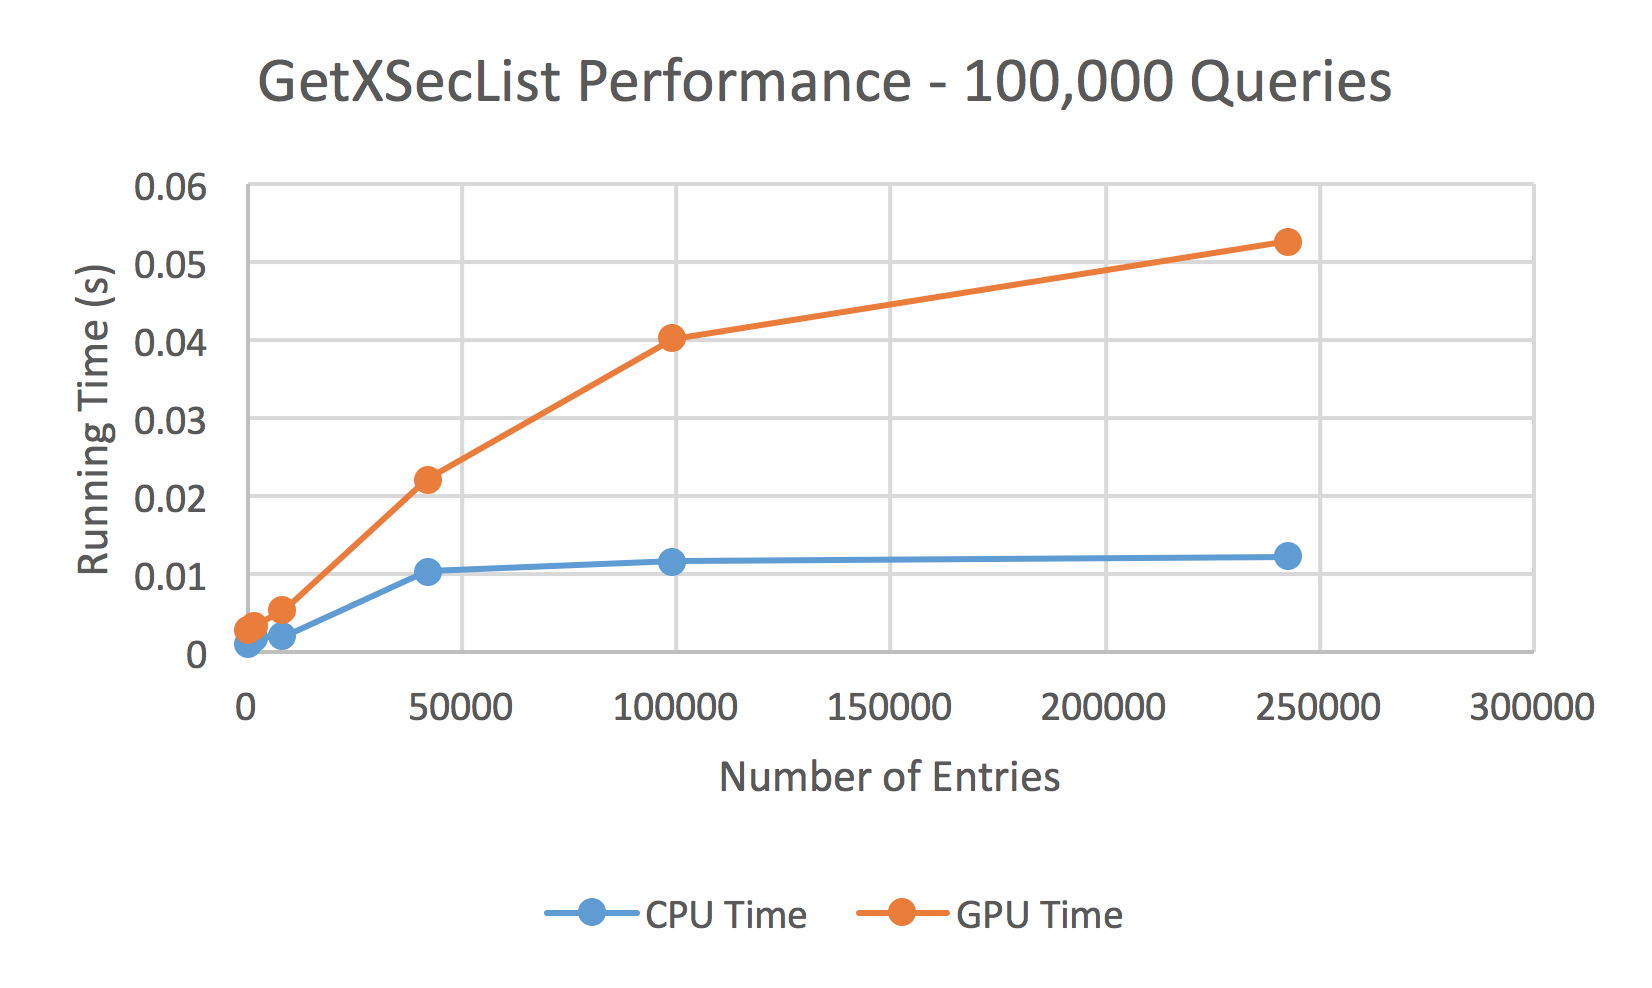
\includegraphics[width=0.8\textwidth]{images/getxseclist_100000.png}
\caption{Runtime vs. Number of Data Points -- \texttt{GetXSecList}, 100,000 Queries}
\end{figure}
\end{frame}

\begin{frame}
\frametitle{Impl. 2: Performance Discussion}
\begin{itemize}
\item CPU implemenation makes use of \texttt{Hash} to quickly find minimum index
\item Finding first element satisfying predicate not well-suited to parallelism
\item If one thread finds element, must wait for all other threads (blocked ifs)
\end{itemize}
\end{frame}

\subsection{Accuracy / Testing}
\begin{frame}
\frametitle{Accuracy}
\begin{itemize}
\item All modified functions except SampleLin and Sample
yield results that precisely match original implementations
\end{itemize}
\begin{itemize}
\item Some functions fell extremely close in accuracy to 
the original, and were considered to 'pass'
\item The average of 1000 SampleLin tests deviated from the 
average of 1000 tests of the original with an error of 0.01 
\end{itemize}
\begin{itemize}
\item The system tests differ if the number of nentries is 
greater than 500; if not however the results of the system 
test conform.
\end{itemize}
\end{frame}

\begin{frame}
\frametitle{Accuracy Discussion}
\begin{itemize}
\item The deviations in SampleLin and Sample can be 
attributed to the functions use of random numbers
\item The negligable deviations in other ported functions 
are likely attributed to differences in CPU and GPU 
arithmetic, leading to different round-off errors
\end{itemize}
\end{frame}

\begin{frame}
\frametitle{Testing}
\begin{itemize}
\item Comparing test results and performance with GPU acceleration enabled and disabled
\item Testing framework based on two phases, one program for each phase
\begin{enumerate}
\item \texttt{GenerateTestResults:} Run unit tests and save results to file
\item \texttt{AnalyzeTestResults:} Compare results from CPU and GPU
\end{enumerate}
\item Run \texttt{GenerateTestResults} once for GPU acceleration enabled, once with it disabled
\end{itemize}
\end{frame}

\begin{frame}[fragile]
\frametitle{\texttt{GenerateTestResults} Details}
\begin{itemize}
\item Includes testing version number in results file for analysis stage
\item Outputs simple results directly to results file
\item For vectors, calculates hash for vector and output it
\item Outputs timing data to separate file
\end{itemize}
\begin{block}{Example: Snippet of Generated Test Results}
\begin{lstlisting}
#void G4ParticleHPVector_CUDA::GetXsecBuffer(
  G4double * queryList, G4int length)_6
@numQueries=10
hash: 16548307878283220284
@numQueries=50
hash: 3204132713354913775
\end{lstlisting}
\end{block}
\end{frame}

\begin{frame}
\frametitle{Demonstration}
\begin{center}
\emph{Demonstration -- Generating Test Results}
\end{center}
\end{frame}

\begin{frame}
\frametitle{\texttt{AnalyzeTestResults} Details}
Two main functions:
\begin{enumerate}
\item Compare results for each test case, printing status to \texttt{stdout}
\begin{itemize}
\item If test failed, output differing values
\item Summarize test results at the end with number passed
\end{itemize}
\item Generate \texttt{.csv} file from timing data
\begin{itemize}
\item One row per unique method call, columns show CPU time, GPU time, method name and parameters
\item Can use Excel to analyze performance results
\end{itemize}
\end{enumerate}
\end{frame}

\begin{frame}
\frametitle{Demonstration}
\begin{center}
\emph{Demonstration -- Analyzing Test Results}
\end{center}
\end{frame}

\section{Conclusion}
\subsection{Summary of Results}
\begin{frame}
\frametitle{Summary of Results}
\begin{itemize}
\item Both Implementations are on average slower than the CPU
\item Most methods slower on GPU until ~10,000 entires in data vector
\item Most commonly-used methods significantly slower on GPU, even with large data vector
\begin{itemize}
\item Lots of data accesses
\end{itemize}
\item SampleLin has accuracy issues due to random number generation
\end{itemize}
\end{frame}

\subsection{Recommendations}
\begin{frame}
\frametitle{Recommendations}
For further work with regards to ParticleHPVector:
\begin{itemize}
\item Abstact further up the Geant4 system, parallelizing 
components that make reference to NeutronHPVector
\item This will decrease the frequency of data transfer 
between the host and device
\item Up-to-date work can be found on out github, along 
with instructions for installing and testing
\end{itemize}
\end{frame}

\begin{frame}
For further work with regards to parallelizing Geant4:
\begin{itemize}
\item Try parallelizing other commonly use components in similar style
\begin{itemize}
\item Look for classes manipulating list-style data structures
\item Classes with functions that have nested loops or are heavy in computing are prime candidates
\item Probabilistic functions and getter/setter functions won't have considerable benefits
\item Functions with conditional branching may cause bottlenecks in parallelization
\end{itemize}
\end{itemize}
\end{frame}

\end{document}
